\chapter{Completed Work}


%%%%%%%%%%%%%%   Overview over article should not include too much equations
%%  bottom line - take home message - the derivations should ref the article

%%  
%%  remove the techinalities - 
%%     using the procedure we have calculated for.. blah blah
%%       see figure. (leave plots only if neccessary to buttom line).
%%
%%  geometry plots - maybe try with normal scale.
%%                   if that doesn't work, leave the figure out.


% Use drawings and slides from the theory lunch (actual and prelim talk)

% Also anything I have in the notes which is worthy.
% For example distance statistics. If I did not contribute, should be in the Appendix.
% Half cooked ideas..

%%%%%%%%%%%%%%%%%%%%%%%%%
\section{The $d=1$ random site model with nearest neighbor hopping}

In $d=1$, a network with randomly distributed sites is equivalent to
an ordered lattice with random transition rates. To make this mapping
we have to know the spacing distribution for this system. We find the
spacing distribution in \autoref{sec:spacing}. A $1d$ lattice with
a known transition rates distribution is exactly solvable \cite{alexander_excitation_1981}.
Basically, it is analogous to adding connectors in series, and 
the diffusion coefficient is the inverse of the combined resistivity
%
\begin{align}
D \ =\ \left(\frac{1}{N} \sum_n \frac{1}{w_{n,n-1}}\right)^{-1}
\end{align}
%
The rates are 
%
\begin{align}
w_{n,n-1} \ =\ w_0 \eexp{-r_{n,n-1}/\xi}
\end{align}
Using the spacing distribution from \autoref{eq:spacing_dist}, we can change distribution variables
from $r$ to $w$. Defining $s \equiv \xi/r_0$ and converting the sum to an integral, we obtain
%
\begin{align}
D \ =\ \left(\frac{1}{N} \int_0^{w_0} \frac{s w^{s-1}dw}{w_0^s}\right)^{-1} \
\ =\ [s>1]\quad \frac{s-1}{s}w_0
\end{align}
% TODO : something is wrong with the N in this expression
This result is valid only for $s>1$. For $s<1$, $D=0$ and we have
subdiffusion, for which the survival probability and spreading 
are also exactly solvable \cite{alexander_excitation_1981}, leading to:
%
\begin{align}
S(t)           \ &\sim \ t^{2s/(1+s)} \\
\mathcal{P}(t) \ &\sim \ t^{-s/(1+s)}
\end{align}
%
The exact results are depicted in \autoref{fig:spread_1d}. 
As explained in \ref{sec:spectrum}, the cumulative spectral distribution
can be deduced from $\mathcal{P}(t)$:
%
\begin{align}
\mathcal{N}(\lambda) \ \sim\ \lambda^{s/(1+s)}
\end{align}
%
Our numerics agree with these results, as seen in the left upper
panel of \autoref{fig:spectral}.

%%%%%%%%%%%
\begin{figure}
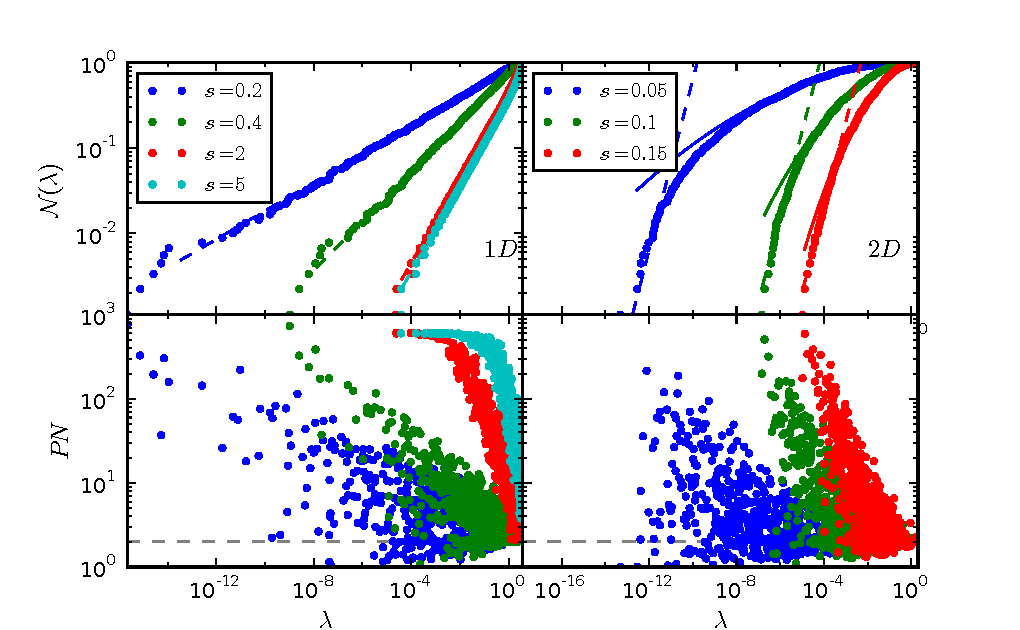
\includegraphics{pts_Spectral_PN.pdf}

\caption{ 
The cumulative eigenvalue distributions $\mathcal{N}(\lambda)$ 
for the $d{=}1$ (1D) and for the $d{=}2$ (2D) degenerate models, 
and the respective PN of the eigenstates (lower panels).
Several representative values of $s$ are considered.
% 
The dots are determined via numerical diagonalization. 
The dashed lines in the upper plots correspond to diffusive behavior.  
%
There is a striking difference between the $d{=}1$ and the $d{=}2$ cases. 
For $d{=}1$, the log-log slope for sparse models ($s<1$) is less than~$d/2$, 
meaning that we have sub-diffusion. In the $d{=}2$ case the small-$\lambda$ log-log slope 
is always~$d/2$, which corresponds to normal diffusion.
%
The horizontal dashed line in the lower panels indicates 
the special value PN$=2$ that corresponds to dimer formation.
}
\label{fig:spectral}
\end{figure}
%%%%

%%%%%%%%%%%%%%%%%%%%%%%%%
\section{The ERH - Effective Range Hopping -procedure}

The diffusion coefficient is defined by the dependence
of the variance in time:
%
\begin{align}
\textrm{Var}(n) \quad =\quad 2d\ D\ t
\end{align}
%
Within the transient diffusion stage,
assuming we start at a specific node $n$, the variance after time
$t$ will be
%
\begin{align}
\textrm{Var}(n) = \sum_m w_{nm} t (x_m-x_n)^2
\end{align}
Therefore, the diffusion coefficient for evolution 
starting at node $n$ is
%
\begin{align}
D_n \quad=\quad \frac{1}{2d}\sum_m (x_m-x_n)^2 w_{nm}
\end{align}
%
Averaging over the starting node, and converting the sum to an integral,
we have
%
\begin{align}\label{eq:linear_D}
D_{\tbox{linear}}  \ \ = \ \ \frac{1}{2d}\iint w(r,\epsilon) \ r^2  \ \rho(r,\epsilon) \ d\epsilon dr 
\end{align}
%

This expression describes the spreading in absence of disorder correctly
for arbitrary long time. However, in a sparse disordered system such as ours,
the possibility of transport is a bit less trivial. Therefore, we suggest
a method to approximate the diffusion, which takes percolation into account.


The basic idea behind \emph{ERH} is that in the linear
expression, nearby sites 
with $r\ll 1$ (and therefore $w \gg 1$ ) are over represented in
the diffusion coefficient calculation. While the transition to
these sites is indeed high, the distance covered is not enough
to form a percolating cluster. Therefore, we use a threshold based
on percolation theory and flat-down the rates higher then this threshold.

The rate threshold $w_c$ is determined using the following expression
%
\begin{align}\label{eq:threshold}
\iint_{w(r,\epsilon)>w_c} \rho(r,\epsilon)drd\epsilon \ \ = \ \ n_c
\end{align}
%
Where $n_c$ is the number of connected sites necessary to form a percolation
cluster.


Next, we suppress the rates higher than $w_c$ to have the value $w_c$,
and use the linear expression \ref{eq:linear_D}, to obtain:
%
\begin{align}\label{eq:ERH_D}
D_{\tbox{ERH}} = \frac{1}{2d}\iint \min\{w(r,\epsilon),w_c\} \ r^2  \ \rho(r,\epsilon) \ d\epsilon dr
\end{align}
%


%%%%%%%%%%%%%%%%%%%%%%%%%
\section{The ERH calculation for several types of network}
%%% This section is actually a collection of subsections.
%%%%%%%%%%%%%%%%%%%%%%%%%%
\subsection{The $d=2$ ordered lattice model, with n.n. hopping}

The model is a  two dimensional grid, with only nearest neighbor hopping possible. 
Each site has $4$ neighbors of equal distance, meaning that
the distribution of sites surrounding each site is simply
%
\begin{align}
\rho(r,\epsilon) \ = \ 4\ f(\epsilon)\delta(r-r_0) 
\end{align}
%
It is well known from percolation theory \cite{stauffer_introduction_1994}
that in this model the number of necessary connections per site is $n_c=2$. We can
find $w_c$ from \ref{eq:threshold},an put this into the ERH 
expression \ref{eq:ERH_D} to have:
%
\begin{align}
D_{\tbox{ERH}} =  \left[\frac{1}{2}w_c + \frac{1}{2}\int_0^{w_c} w\tilde{f}(w) dw\right]r_0^2
\end{align}
%
Where we converted the $f(\epsilon)d\epsilon$ integral to a $\tilde{f}(w)dw$
integral. In absence of the disorder (i.e.\ all the rates are equal),
the known result $D = w_0r_0^2$ is restored.


%%%%%%%%%%%%%%%%%%%%%%%%%%
\subsection{The degenerate hopping model}

In this model the sites are randomly distributed in a $d$ dimensional 
space, all with $\epsilon=0$. Every site is connected to all of the other
sites, with the transition rates according to \ref{eq:random_hopping_rates}.

Since $w$ depends only on $r$, we may define the ERH threshold by
$r_c$ instead of $w_c$. Rephrasing equation \ref{eq:threshold}, and 
using $\rho(r,\epsilon)$ from \ref{eq:site_distribution}, $r_c$ is determined according to
%
\begin{align}
\int_0^{r_c} \frac{\Omega_d r^{d-1} dr}{r_0^2} \ = \  n_c 
\end{align}
%
With the simple solution:
%
\begin{align}
r_c  &\equiv \left(\frac{d}{\Omega_c}n_c\right)^{1/d}  r_0 \\
w_c &= w_0\exp\left(-\frac{r_c}{\xi}\right) 
\end{align}
%

Now we shall put all of the above into the ERH expression \ref{eq:ERH_D}.
The solution involves the incomplete gamma function \cite{_nist_????},
%
\begin{align}
\Gamma(\ell{+}1,x) = \int_0^x r^{\ell} \eexp{-r} dr = 
\ell! \ \mbox{EXP}_{\ell}(x)  \ \eexp{-x}
\end{align}
%
And the polynomial
%
\begin{align}\label{eq:EXP}
\mathrm{EXP}_{\ell}(x) \ \ = \ \ \sum_{k=0}^{\ell} \frac{1}{k!} \, x^k
\end{align}
% 
The integral is only over $dr$, and it is split  
into the domains ${0<r<r_c}$ and ${r>r_c}$. 
Namely, 
%
\begin{align}
D_{\tbox{ERH}} &= 
\frac{w_0\Omega_d}{2d}\int_0^{r_c} \eexp{-r_c / \xi} \frac{r^{d+1}}{r_0^d} dr 
\nonumber 
\quad+\quad \frac{w_0\Omega_d}{2d}\int_{r_c}^\infty \eexp{-r / \xi} \frac{r^{d+1}}{r_0^d} dr 
\nonumber \\
&= \frac{w_0\Omega_d}{2d} \eexp{-r_c / \xi} \frac{r_c^{d+2}}{d+2} \frac{1}{r_0^d}
\nonumber 
\quad+\quad \frac{w_0\Omega_d}{2d} \frac{\xi^{d+2}}{r_0^d} \Gamma\left(d+2,\frac{r_c}{\xi}\right)
\nonumber \\
&= \frac{w_0\Omega_d \xi^{d+2}}{2d(d+2)r_0^d}\Gamma\left(d+3,\frac{r_c}{\xi}\right)\\
&= \mathrm{EXP}_{d{+}2}\left(\frac{1}{s_c}\right)  \  \eexp{-1/s_c}  \ D_{\tbox{linear}}
\end{align}
%
Where $s_c=\xi/r_c$, and $D_{\tbox{linear}}$ is formally obtained by setting
$r_c=0$ in $D_{\tbox{ERH}}$  i.e.:
%
\begin{align}\label{eq:D_linear}
D_{\tbox{linear}} \ \ = \ \  
\frac{(d{+}1)!\,\Omega_d}{2d} \, s^{d{+}2} \, w_0 r_0^2
\end{align}

The ERH result depends on $n_c$, the number of bonds 
required for percolation.
For $d=2$, we have used the $n_c=4.5$ result from \cite{dalton_dependence_1964,*pike_percolation_1974}, 
and compared it with our numerics in figure \ref{fig:spread_2d}.

\begin{figure}
\begin{subfigure}{0.4\textwidth}
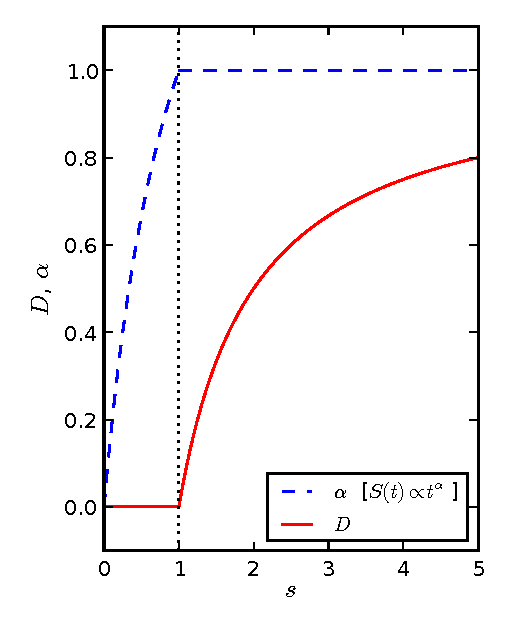
\includegraphics[scale=0.7]{ptsD_1D_long}
\caption{Spreading in $d{=}1$}
\label{fig:spread_1d}
\end{subfigure}
\begin{subfigure}{0.48\textwidth}
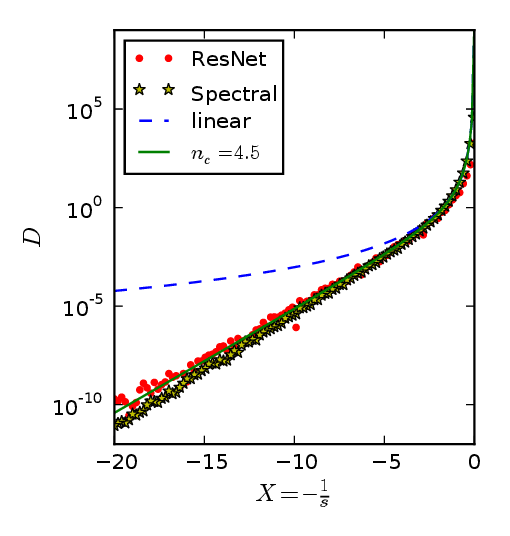
\includegraphics{ptsD_2D_long}
\caption{Spreading in $d{=}2$}
\label{fig:spread_2d}
\end{subfigure}
\caption{In \subref{fig:spread_1d} the red line is the diffusion coefficient $D$. It is zero in the sub-diffusive regime $s<1$. 
The blue dashed line is the power of the spreading, showing sub-diffusive behavior for $s<1$.
In \subref{fig:spread_2d} the green line represents the ERH estimate with $n_c=4.5$, while the dashed blue line stands for
the linear estimate. The red dots are based on numerical resistor network calculation, while the stars are extracted from the
spectral analysis. }
\end{figure}



%%%%%%%%%%%%%%%%%%%%%%%%%%%%
\subsection{The Mott hopping model}

For the Mott hopping model, with rates according to \autoref{eq:mott_hopping_rates},
and rate distribution according to \autoref{eq:mott_distribution}, the ERH 
threshold is determined using \autoref{eq:threshold}:
%
\begin{align}
\epsilon_c &\equiv \left( \frac{d}{\Omega_d} \frac{n_c}{s^d} \right)^{1/(d+1)} \\
w_c &= w_0\exp(-\epsilon_c) 
\end{align}
%
This integral has two dimensions, $dr$ and $d\epsilon$,
split into two domains 
${w>w_c}$ and ${0<w<w_c}$. The two domains are 
separated by the line ${\epsilon+(r/\xi)=\epsilon_c}$ which is illustrated in \autoref{fig:wdiagram}.

\begin{figure}
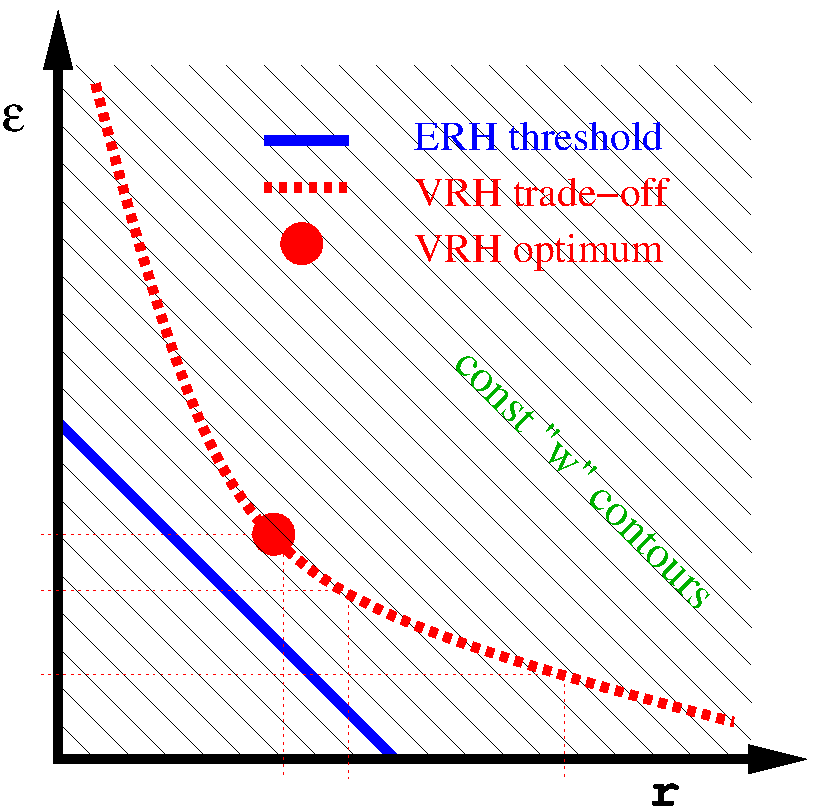
\includegraphics[scale=0.6]{wdiagram}
\caption[VRH vs ERH]{Comparing VRH with ERH. The thin black lines 
correspond to equal rates. The solid blue line corresponds to the
ERH threshold $w_c$, while the red dashed line corresponds to the
VRH trade-off. The red dot is the VRH optimum point, used for the
VRH calculation.}
\label{fig:wdiagram}
\end{figure}


It is therefore natural to change variables:
%
\begin{align}
x\ \ &= \ \ \epsilon+(r/\xi) \\
y\ \ &= \ \ \frac{1}{2}\left(-\epsilon+(r/\xi)\right) 
\end{align}
%
hence 
%
\begin{align}
D_{\tbox{ERH}} &= 
\frac{w_0\Omega_d}{2dr_0^d}\int_0^{\epsilon_c}\! \xi dx \int_{-x/2}^{x/2} \! dy \, \eexp{-\epsilon_c} \left(\xi y + \xi \frac{x}{2}\right)^{d+1} 
\nonumber \\
& + \frac{w_0\Omega_d}{2dr_0^d}\int_{\epsilon_c}^{\infty} \! \xi dx \int_{-x/2}^{x/2} \! dy \, \eexp{-x} \left(\xi y+\xi \frac{x}{2}\right)^{d+1} 
\nonumber \\
&= \frac{w_0\Omega_d}{2dr_0^d}\xi^{d+2} \eexp{-\epsilon_c} \frac{\epsilon_c^{d+3}}{(d+2)(d+3)}  
\nonumber \\
& +\frac{w_0\Omega_d}{2dr_0^d(d+2)}\xi^{d+2} \Gamma\left(d+3,\epsilon_c\right)
\nonumber \\
&= \frac{w_0\Omega_d \xi^{d+2}}{2d(d+2)(d+3)r_0^d}\Gamma\left(d+4,\epsilon_c\right) \nonumber\\
&=\mathrm{EXP}_{d{+}3}\left(\epsilon_c\right)  \  \eexp{-\epsilon_c}  \ D_{\tbox{linear}}
\end{align}
%
With $\mathrm{EXP}_\ell$ and $D_{\tbox{linear}}$ the same as in 
\autoref{eq:EXP} and \autoref{eq:D_linear}.




%%%%%%%%%%%%%%%%%%%%%%%%%%%
\subsection{The quasi one dimensional model}\label{sec:quasi_oned}

This model is a Banded one dimensional lattice model. Each site 
is connected to $b$ other sites, the disorder arising from
variations in $\epsilon$. 
We find the ERH threshold from \autoref{eq:threshold}:
%
\begin{align}\label{eq:thres_banded}
\int_0^{\infty}  
\frac{2 dr}{r_0} 
\ F\left(\log\left(\frac{w_0}{w_c}B(r)\right)\right) 
\ \ = \ \ n_c
\end{align}
%
Where $F(\epsilon)$ is the cumulative distribution function, or the integral of $f(\epsilon)$.


For now, we shall assume a flat profile,
%
\begin{align}
B(r) = \begin{cases}
1 & \text{if } r <= b \\
0 & \text{if } r>b
\end{cases}
\end{align}
%
Together with a uniform distribution of $\epsilon$ over $[0,\sigma]$, which means that the rates are log-uniform distributed. Large $\sigma$ corresponds 
to a very wide distribution of rates, meaning a "sparse" system (see 
\autoref{sec:sparsity}).

Note that even with large $\sigma$, the distribution has a lower non zero bound, meaning that the system is still diffusive.


We continue our threshold seeking from \autoref{eq:thres_banded}, using this 
flat profile, and find $\epsilon_c$ to be:
%
\begin{align}
2b\ F(\epsilon_c) \ =\ n_c \\
\epsilon_c\ = \ \frac{n_c}{2b}\sigma
\end{align}
%
The ERH integral (\autoref{eq:ERH_D} )is replaced by a sum, leading to
\begin{align}
D_{\text{ERH}} \ \ = \ \ 
\ \frac{1}{\sigma}\left[ 
\left(1+\frac{n_c}{2b}\sigma\right)\eexp{-\frac{n_c}{2b}\sigma} - \eexp{-2\sigma}
\right] \ \tilde{b} w_0
\end{align}
Where we have defined
%
\begin{align}
\tilde{b} \ \ \equiv \ \ \sum_{r=1}^b r^2 \ \ = \ \ = \frac{1}{6}b(b+1)(2b+1)
\end{align}
%
As before, the linear result is formally obtained by setting $n_c=0$.

This result is compared to numerical computation in \autoref{fig:banded}.

%%%%%%%%%%%%%%
\begin{figure}
\begin{subfigure}{0.49\textwidth}
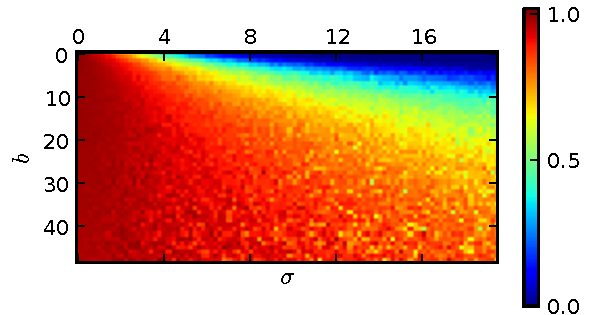
\includegraphics[width=\hsize]{ptsD_banded_Image}
\subcaption{Several values of $b$ and $\sigma$}\label{fig:band_image}
\end{subfigure}
\begin{subfigure}{0.49\textwidth}
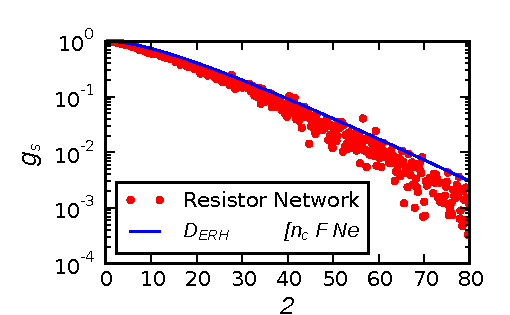
\includegraphics[width=\hsize]{ptsD_banded}
\subcaption{For $b=10$ only.}\label{fig:band_b10}
\end{subfigure}
\caption[Banded network]{Numerics Vs ERH estimation for the quasi one dimensional network. $g_s = D/D_{\tbox{linear}}$ is plotted on both graphs.
On \subref{fig:band_b10}, the blue line is the ERH estimation. If the
linear result was correct, $g_s$ would have been $1$ for all values of $\sigma$.}
\label{fig:banded}
\end{figure}



%%%%%%%%%%%%%%%%%%%%%%%%%%%%%%%%%%%%%%%%%%%%%
\section{Geometrical implications}


For the $2d$ stochastic model, we wanted to verify the fact that
the geometry of the model has more effect than simply dictating the distribution
of the rates. To achieve this, we have constructed the matrix as usual, but
then shuffled the matrix elements randomly (within the upper triangle). That way
we assured that the distribution of elements stays the same, while the topological
and geometrical relations between sites is dismantled. After symmetrization
and resetting of the main diagonal, we have numerically diagonalized the matrix. The
results can be seen in \autoref{fig:rand}.


\begin{figure}
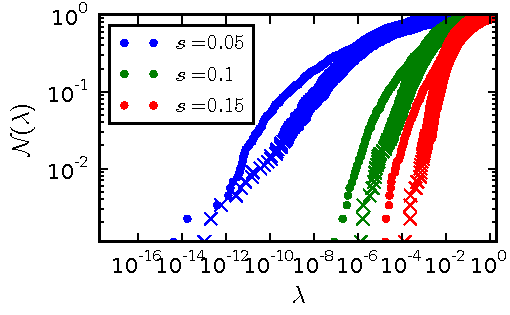
\includegraphics{pts_geom}
\caption{Changes in the spectrum due to randomization of the rates. The solid circles 
  stand for the regular spectrum, and the crosses for the randomized matrix.}
\label{fig:rand}
\end{figure}


%%%%%%%%%%%%%%%%%%%%%%%%%%%%%%%%%%%%%%%%%%%%%%%%%%%%
%%%%%%%%%%%%%%%%%%%%%%%%%%%%%%%%%%%%%%%%%%%%%%%%%%%%
\chapter{Preliminary analysis}


%%%%%%%%   Daniel's RP has better preliminary. 

%%%%%%%%   I need to add dts.tex here.
%%%%%%%%   I could also add D(g_s) and say that it failed

%%%%%%%%%%%%%%%%%%%%%%%%%%%%%
\section{The quasi one dimensional Hamiltonian}


In this model , described in \autoref{sec:quasi_bg}, initial analysis of
the numerical results reveals that the sparsity affects the diffusion coefficient.
We see that as the system becomes more sparse, the diffusion coefficient is suppressed. 
As might be expected, the lower bandwidth ensembles are more
susceptible, as the system is more vulnerable to disconnections.



\begin{figure}
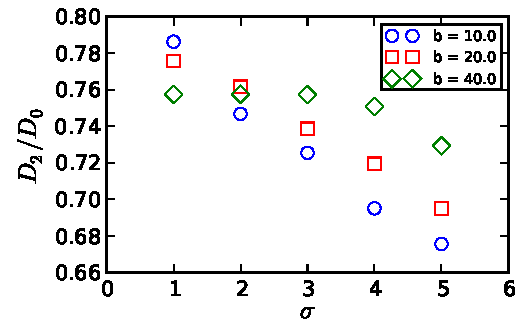
\includegraphics{dts_D2}
\caption{The transient diffusion coefficient for quantum spreading in
a banded sparse network. The ratio $D/D_0$ between the numerical diffusion 
coefficient and the expected value decreases as $\sigma$ increases. The effect
is stronger for low bandwidth.}
\end{figure}
